%Incidencia de una onda plana a 45° con n_i = 1, n_t = 1.46   

\documentclass[tikz,border=1cm]{standalone}

\usepackage{tikz}
\usetikzlibrary{decorations.pathreplacing,decorations.pathmorphing}

\begin{document}


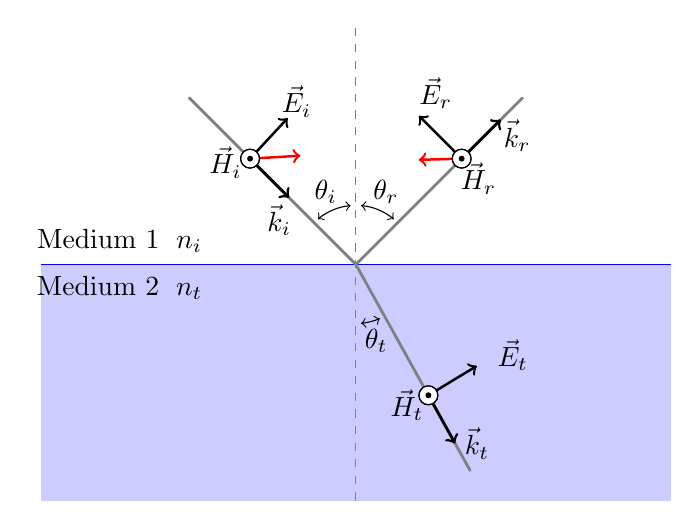
\begin{tikzpicture}%[   ESTO PONE LAS RAYAS QUE USO EN EPSEJOS
%    interface/.style={
        % The border decoration is a path replacing decorator. 
        % For the interface style we want to draw the original path.
        % The postaction option is therefore used to ensure that the
        % border decoration is drawn *after* the original path.
%        postaction={draw,decorate,decoration={border,angle=-45,
%                    amplitude=0.3cm,segment length=2mm}}},
%    ]



%-------------------------------------------- Incidence media
\fill[blue!20] (-4,-3) rectangle (4,0);
% Interface
\draw[blue,line width=.5pt](-4,0)--(4,0); %%..5pt, interface]
% Vertical dashed line
\draw[dashed,gray,](0,-3)--(0,3);
% Media names
\node at (-3,.3) {Medium 1 $\; n_i$}; 
\node at (-3,-.3) {Medium 2 $\; n_t$};

%--------------------------------------------  Incident Wave
\draw[gray, line width=1pt](0:0cm)--(135:3cm);  % Light trajectory
\path (0,0)++(112.5:1cm)node{$\theta_i$};       % Angle
\draw[<->](95:.75cm)arc(95:130:.75cm);
 
    \draw[->,line width=1pt](135:1.9cm)--(135:1.2cm);    %Wave vector
    \path (0,0)++(141:0.9cm)node[left]{$\vec{k}_i$};     %Wave vector label
    
    \draw[->,line width=.9pt](135:1.9cm)--(115:2.05cm);  %E vector
    \path (0,0)++(110:2.2cm)node{$\vec{E}_i$}; 
    \draw[->,line width=.9pt, red]((135:1.9cm)--(117:1.55cm); 

    
    \path (0,0)++(142:2.1cm)node{$\vec{H}_i$};       % B vector
    
    \draw [fill= white](135:1.9cm)circle (0.12cm);
    \draw [black](135:1.9cm)circle (0.12cm);
    \filldraw[fill=black](135:1.9cm) circle(0.03cm); %%    
    
    
%    \draw[line width=.6pt] (135:1.9cm)   % Esto esra paea hacer el vector salir de la hoja
%                         +(-135:.12cm) -- +(45:.12cm)
%                         +(-45:.12cm) -- +(135:.12cm);    
   
    
%--------------------------------------------  Reflected Wave
\draw[gray,line width=1pt](0:0cm)--(45:3cm);  % Light trajectory
\path (0,0)++(67.5:1cm)node{$\theta_r$};       % Angle
\draw[<->](85:.75cm)arc(85:50:.75cm);
 
    \draw[->,line width=1pt](45:1.9cm)--(45:2.6cm);    %Wave vector
    \path (0,0)++(43:2.4cm)node[right]{$\vec{k}_r$};     %Wave vector label
    
    \draw[->,line width=.9pt](45:1.9cm)--(67:2.05cm);  %E vector
    \path (0,0)++(65:2.4cm)node{$\vec{E}_r$};
    \draw[->,line width=.9pt, red](45:1.9cm)--(59:1.55cm); 
   % \draw[dashed,red,line width=.9pt](59:1.55cm)--(67:2.05cm);
    
    \path (0,0)++(35:1.9cm)node{$\vec{H}_r$};       % B vector
    
    \draw [fill= white](45:1.9cm)circle (0.12cm);
    \draw [black](45:1.9cm)circle (0.12cm);
    \filldraw[fill=black](45:1.9cm) circle(0.03cm); %%  


%--------------------------------------------  Transmitted Wave
\draw[gray,line width=1pt](0:0cm)--(-61:3cm);  % Light trajectory
\path (0,0)++(-75:1cm)node{$\theta_t$};       % Angle
\draw[<->](-85:0.75cm)arc(-85:-66:.75cm);
 
    \draw[->,line width=1pt](-61:1.9cm)--(-61:2.6cm);    %Wave vector
    \path (0,0)++(-61:2.6cm)node[right]{$\vec{k}_t$};     %Wave vector label

    \draw[->,line width=.9pt](-61:1.9cm)--(-40:2.005cm);  %E vector
    \path (0,0)++(-30:2.3cm)node{$\vec{E}_t$}; 
    
    \path (0,0)++(-70:1.9cm)node{$\vec{H}_t$};       % B vector
    
    \draw [fill= white](-61:1.9cm)circle (0.12cm);
    \draw [black](-61:1.9cm)circle (0.12cm);
    \filldraw[fill=black](-61:1.9cm) circle(0.03cm); %%  
 

\end{tikzpicture}
\end{document}